% Memoria de la Práctica 1 de PLN I (Universitat d'Alacant), formato ACL.
% Compilar:  tectonic memoria.tex   (o pdflatex + bibtex, o subir la carpeta a Overleaf)
% Todas las cifras salen de results/, runs/ y de los tests del repositorio.
\documentclass[11pt]{article}
\usepackage[final]{acl}
\usepackage{times}
\usepackage{latexsym}
\usepackage[T1]{fontenc}
\usepackage[utf8]{inputenc}
\usepackage[spanish,es-tabla,es-nodecimaldot,es-noshorthands]{babel}
\usepackage{microtype}
\usepackage{inconsolata}
\usepackage{graphicx}
\usepackage{booktabs}
\usepackage{amsmath}
\usepackage{amssymb}
\usepackage{xcolor}
\usepackage{etoolbox}
\patchcmd{\thebibliography}{References}{Referencias}{}{}
\patchcmd{\thebibliography}{{References}}{{Referencias}}{}{}
\patchcmd{\thebibliography}{{References}}{{Referencias}}{}{}

\newcommand{\TODO}[1]{\textcolor{red}{[#1]}}
\newcommand{\pmsd}[1]{{\scriptsize$\pm$#1}}

\title{Ampliación del GPT de Raschka con codificaciones posicionales\\y Mixture of Experts}

\author{Alejandro Operé \quad David Muñoz \quad Elena Fernández \quad María Mestre \\
  Procesamiento del Lenguaje Natural I, Grado en Ingeniería en Inteligencia Artificial \\
  Universitat d'Alacant}

\begin{document}
\maketitle

\begin{abstract}
En esta práctica hemos ampliado el GPT que se construye en los capítulos 2 a 6 de \citet{raschka2024build} con dos técnicas de los LLM actuales.
La primera cambia la forma en que el modelo codifica la posición de cada token (APE aprendida y sinusoidal, NoPE, ALiBi, el sesgo relativo de T5 y un híbrido por capas) y estudia qué pasa cuando las secuencias son más largas que las de entrenamiento.
La segunda sustituye la capa feed-forward de cada bloque por una capa Mixture of Experts (MoE), en la que un router decide qué expertos procesan cada token.
Comprobamos las implementaciones comparándolas numéricamente con PyTorch y con Hugging Face, y las evaluamos entrenando modelos pequeños desde cero con Tiny Shakespeare.
ALiBi mantiene la perplejidad con secuencias 8 veces más largas que las de entrenamiento, y el MoE mejora la entropía cruzada en 0.05 nats sin aumentar el cálculo por token.
Al juntar las dos ampliaciones, el MoE mejora con todas las codificaciones, pero solo conserva la mejora en secuencias largas con ALiBi.
\end{abstract}

\section{Introducción}
El GPT del libro usa una codificación posicional absoluta aprendida (una tabla con un vector por posición) y una capa feed-forward (FFN) densa en cada bloque.
Los LLM recientes han cambiado las dos cosas \citep{raschka2025comparison}.
Muchos usan codificaciones relativas, o directamente ninguna, para poder trabajar con contextos más largos que los de entrenamiento.
Otros reparten la capa FFN entre varios expertos para tener más parámetros sin hacer más cálculos por token \citep{shazeer2017outrageously,lepikhin2021gshard,fedus2022switch,jiang2024mixtral}.

En este trabajo hemos implementado ambas ideas sobre el modelo del libro (secciones \ref{sec:pe} y \ref{sec:moe}) y después las hemos juntado en un mismo modelo (sección \ref{sec:combo}).
Las ampliaciones se activan por configuración, sin modificar el código base, y las hemos comprobado con 111 tests automáticos y 176 comprobaciones adicionales.
RoPE \citep{su2024roformer} no forma parte de nuestras ampliaciones porque el profesor la descartó, así que solo la usamos como referencia.

\section{Modelo base y experimentos}
\label{sec:base}
Usamos el GPT del libro (con la normalización antes de cada subbloque, como GPT-2) en una versión pequeña: 4 capas, dimensión 128, 4 cabezas de atención y un contexto de 128 tokens, en total unos 0.82M de parámetros.
Lo entrenamos desde cero a nivel de carácter con Tiny Shakespeare \citep{karpathy2015charrnn}, que tiene 1.1M caracteres y 65 símbolos distintos.
Usamos el 90\% del texto para entrenar y el 10\% para validar, con AdamW (tasa de aprendizaje $10^{-3}$ y decaimiento de pesos 0.1) y lotes de 32.
Todo se entrenó en CPU, y cada experimento se repitió con 3 semillas.
Usamos dos montajes. En el \textbf{P1} (codificaciones posicionales) entrenamos 5 épocas con ventanas de 128 tokens (unos 1225 pasos) y dropout 0.1, y después medimos la perplejidad con ventanas de 32 a 1024 tokens, es decir, hasta 8 veces más largas que en entrenamiento, puntuando solo los últimos 32 tokens de cada ventana.
En el \textbf{P2} (MoE) entrenamos 2000 pasos con trozos aleatorios del texto (8.2M tokens) y sin dropout, y medimos la entropía cruzada (CE, en nats) sobre 20 lotes fijos de validación.
En las tablas damos la media y la desviación típica entre semillas.

\section{Codificaciones posicionales}
\label{sec:pe}
\paragraph{Implementación.}
Hemos preparado el modelo para que la codificación posicional se pueda cambiar sin tocar el resto.
Hay tres sitios donde puede actuar: sumando un vector a la entrada (las codificaciones absolutas), girando las consultas y las claves (RoPE) o sumando un sesgo a las puntuaciones de la atención (ALiBi y T5).
En general, la puntuación de la cabeza $h$ entre la consulta $i$ y la clave $j\le i$ queda
\begin{equation}
s^h_{ij} = \frac{(R_i q_i)^\top (R_j k_j)}{\sqrt{d_h}} + b_h(i-j),
\end{equation}
antes de aplicar la máscara causal y el softmax.
La versión sinusoidal \citep{vaswani2017attention} calcula el vector de cada posición con senos y cosenos, así que existe para cualquier posición.
NoPE no usa ninguna codificación: el modelo solo conoce el orden por la máscara causal \citep{kazemnejad2023impact}.
ALiBi resta a cada puntuación una cantidad proporcional a la distancia, $b_h(\Delta) = -m_h \Delta$, con una pendiente $m_h = 2^{-8h/H}$ distinta en cada cabeza \citep{press2022alibi}.
T5 aprende un sesgo por cabeza y por rango de distancias: 16 distancias exactas y 16 rangos logarítmicos hasta 128 \citep{raffel2020t5}.
Por último, el híbrido quita RoPE en una de cada $N$ capas \citep{yang2025rope}.

\paragraph{Comprobaciones.}
Para asegurarnos de que la atención está bien, la comparamos con la de PyTorch \citep{paszke2019pytorch} con las mismas entradas. En el caso de RoPE y T5 también la comparamos con Hugging Face \citep{wolf2020transformers}.
Además, con los pesos del modelo base, el modelo nuevo da los mismos logits que el original (Tabla~\ref{tab:val}).

\begin{table}[t]
\centering\small\setlength{\tabcolsep}{2.8pt}
\begin{tabular}{@{}lccccc@{}}
\toprule
 & CE val & \multicolumn{4}{c}{Perplejidad (últimos 32 tokens)} \\
\cmidrule(l){3-6}
Codificación & ctx 128 & 128 & 256 & 512 & 1024 \\
\midrule
APE aprendida & 1.820 & 6.02 & 23.73 & 22.15 & --$^a$ \\
APE sinusoidal & 1.813 & 5.88 & 23.17 & 24.42 & 23.09 \\
NoPE & 2.011 & 7.50 & 11.03 & 13.32 & 13.94 \\
ALiBi & 1.757 & 5.57 & \textbf{5.58} & \textbf{5.58} & \textbf{5.59} \\
T5 & 1.772 & 5.67 & 6.34 & 9.40 & 13.46 \\
\midrule
\textcolor{gray}{RoPE (ref.)} & \textcolor{gray}{1.677} & \textcolor{gray}{5.07} & \textcolor{gray}{13.90} & \textcolor{gray}{24.57} & \textcolor{gray}{42.03} \\
\textcolor{gray}{Híbrido, $N{=}4$} & \textcolor{gray}{1.698} & \textcolor{gray}{5.20} & \textcolor{gray}{15.97} & \textcolor{gray}{27.09} & \textcolor{gray}{43.92} \\
\bottomrule
\end{tabular}
\caption{Montaje P1: entrenando con contexto 128 y evaluando hasta 1024. Media de 3 semillas; la desviación es como mucho 0.011 en CE y 1.8 en perplejidad (hasta 6.8 en RoPE y el híbrido). $^a$En estas ejecuciones la tabla de posiciones tenía 512 filas.}
\label{tab:pe}
\end{table}

\paragraph{Resultados.}
En la Tabla~\ref{tab:pe} se ve que las codificaciones absolutas fallan en cuanto la secuencia pasa de los 128 tokens de entrenamiento: la perplejidad se multiplica por cuatro.
ALiBi es la única que no empeora nada hasta 1024 tokens (de 5.57 a 5.59), aunque con contexto 128 queda algo por detrás de RoPE.
T5 empeora poco a poco, y NoPE empeora menos en proporción, pero ya parte de la peor perplejidad.
RoPE es la mejor con el contexto de entrenamiento y la peor con 1024, y el híbrido no lo arregla con un modelo tan pequeño.

También probamos tareas algorítmicas (Tabla~\ref{tab:tasks}), entrenando con secuencias de hasta 20 elementos y evaluando con secuencias de 21 a 40.
Las codificaciones absolutas prácticamente no generalizan, NoPE ordena perfectamente y ALiBi es la mejor copiando y en la paridad, igual que en \citet{kazemnejad2023impact}.
La suma, la suma módulo 10 y el recuerdo asociativo no llegaron a aprenderse ni con las longitudes de entrenamiento (como mucho un 33\% de acierto), así que no sirven para comparar.

\begin{table}[t]
\centering\small\setlength{\tabcolsep}{3.5pt}
\begin{tabular}{@{}lcccccc@{}}
\toprule
Tarea & Apr. & Sin. & NoPE & ALiBi & T5 & \textcolor{gray}{RoPE} \\
\midrule
Copiar & 0.00 & 0.00 & 0.21 & \textbf{0.50} & 0.14 & \textcolor{gray}{0.04} \\
Invertir & 0.00 & 0.00 & \textbf{0.29} & 0.13 & 0.14 & \textcolor{gray}{0.05} \\
Ordenar & 0.00 & 0.22 & \textbf{1.00} & 0.49 & 0.79 & \textcolor{gray}{0.10} \\
Paridad & 0.51 & 0.50 & 0.52 & \textbf{0.61} & 0.47 & \textcolor{gray}{0.49} \\
\bottomrule
\end{tabular}
\caption{Acierto en longitudes no vistas (media de 3 semillas). Con las longitudes de entrenamiento el acierto es 1.00, salvo en paridad (de 0.67 a 0.99).}
\label{tab:tasks}
\end{table}

\section{Mixture of Experts}
\label{sec:moe}
\paragraph{Implementación.}
En cada bloque cambiamos la capa FFN por $E$ expertos, cada uno igual que el FFN original, y un router lineal que decide qué $k$ expertos procesan cada token $x$:
\begin{equation}
\begin{gathered}
p = \mathrm{softmax}(W_r x)\in\mathbb{R}^E,\qquad \mathcal{T} = \mathrm{top}_k(p),\\
y = \textstyle\sum_{e\in\mathcal{T}} w_e\,\mathrm{FFN}_e(x).
\end{gathered}
\end{equation}
Cuando $k>1$ normalizamos los pesos de los expertos elegidos para que sumen 1, como en Mixtral \citep{jiang2024mixtral}.
Con $k=1$ usamos directamente la probabilidad, como en Switch Transformer \citep{fedus2022switch}: si la normalizáramos, el peso valdría siempre 1 y el router no aprendería nada de la pérdida principal. Lo comprobamos: su gradiente pasa de 19.6 a prácticamente 0.

Para que el router no mande casi todo a unos pocos expertos, añadimos la pérdida de balanceo de Switch Transformer:
\begin{equation}
\mathcal{L}_{\mathrm{aux}} = E \textstyle\sum_{i=1}^{E} f_i P_i,\qquad \mathcal{L} = \mathrm{CE} + \alpha\,\mathcal{L}_{\mathrm{aux}},
\end{equation}
donde $f_i$ es la fracción de tokens asignados al experto $i$ y $P_i$ la probabilidad media que le da el router.
Vale 1 si el reparto es uniforme y $E$ si todo va al mismo experto, y la promediamos entre capas.

Para que el MoE sea rápido, en vez de pasar todos los tokens por todos los expertos, ordenamos los tokens según el experto que les toca.
Así cada experto procesa de una vez todos sus tokens, y después cada resultado vuelve a su posición, sumando los de sus $k$ expertos.
De esta forma el coste depende de $k$ y no del número de expertos.

\begin{table}[t]
\centering\footnotesize\setlength{\tabcolsep}{3pt}
\begin{tabular}{@{}p{6.1cm}r@{}}
\toprule
Comprobación & Dif. máx. \\
\midrule
Atención (NoPE/ALiBi/RoPE) frente a PyTorch & $\le10^{-5}$ \\
RoPE y sesgo de T5 frente a HF & 0 \\
Modelo nuevo frente al GPT del libro & $\le10^{-6}$ \\
MoE frente a Mixtral (HF) & $8\cdot10^{-7}$ \\
MoE con $k{=}1$ frente a Switch Transformer (HF) & 0 \\
Pérdida de balanceo y z-loss frente a HF & $\le10^{-6}$ \\
MoE rápido frente al lento (con gradientes) & $\le10^{-5}$ \\
MoE con un experto frente al FFN del libro & $\le10^{-5}$ \\
GPT con expertos copiados frente al GPT denso & $\le10^{-5}$ \\
Pérdida inyectada frente a sumarla a mano & $\le10^{-6}$ \\
\bottomrule
\end{tabular}
\caption{Comparaciones numéricas con las mismas entradas (HF: Hugging Face).}
\label{tab:val}
\end{table}

\paragraph{Comprobaciones.}
Comparamos nuestra capa con las versiones de Hugging Face de Mixtral (con expertos SwiGLU, como en el original) y de Switch Transformer, copiando los mismos pesos, y las salidas coinciden (Tabla~\ref{tab:val}).
La pérdida de balanceo también coincide con la de Hugging Face, salvo un factor $k$, porque nosotros la normalizamos para que 1 signifique reparto equilibrado sea cual sea $k$.
También comprobamos que con un solo experto la capa es exactamente el FFN del libro, y que un GPT con todos los expertos copiados del FFN original \citep{komatsuzaki2023upcycling} da los mismos logits que el modelo base.

\begin{table}[t]
\centering\small\setlength{\tabcolsep}{2.5pt}
\begin{tabular}{@{}lcccc@{}}
\toprule
Modelo & Parám. (act.) & CE val & tok/s & Carga \\
\midrule
Denso (libro) & 0.82M & 1.645\pmsd{.008} & 18.6k & -- \\
MoE $k{=}1$ & 2.41M (0.83M) & 1.595\pmsd{.012} & 17.6k & 0.34 \\
MoE $k{=}2$ & 2.41M (1.35M) & 1.581\pmsd{.006} & 11.9k & 0.31 \\
Denso ancho & 2.40M & 1.576\pmsd{.004} & 6.4k & -- \\
\midrule
$k{=}1$, $\alpha{=}0$ & 2.41M (0.83M) & 1.605\pmsd{.006} & 17.5k & 0.65 \\
$k{=}1$, $\alpha{=}0.1$ & 2.41M (0.83M) & 1.594\pmsd{.004} & 17.9k & 0.26 \\
$k{=}1$, z-loss & 2.41M (0.83M) & 1.596\pmsd{.010} & 16.0k$^\dagger$ & 0.35 \\
\bottomrule
\end{tabular}
\caption{Montaje P2 con 4 expertos y $\alpha{=}0.01$, salvo que se indique otra cosa. El denso ancho tiene un FFN 4 veces más ancho. Carga: fracción de tokens que recibe el experto más usado en la peor capa (0.25 sería un reparto perfecto). $^\dagger$Medido otro día, no comparable.}
\label{tab:moe}
\end{table}

\paragraph{Resultados.}
Con $k=1$, el MoE hace el mismo cálculo por token que el modelo denso y baja la CE en 0.050 nats: las 3 semillas del MoE son mejores que las 3 del denso. Además, solo entrena un 5.6\% más despacio (Tabla~\ref{tab:moe}).
También lo comparamos con un modelo denso con los mismos parámetros totales, que tiene un FFN 4 veces más ancho y por tanto hace mucho más cálculo.
El MoE con $k=1$ consigue el 72\% de su mejora y entrena 2.75 veces más rápido; con $k=2$ consigue el 93\% y entrena 1.86 veces más rápido.

Sin la pérdida de balanceo, el experto más usado llega a recibir el 65\% de los tokens (Figura~\ref{fig:main}c), y con $\alpha=0.1$ el reparto es casi perfecto (26\%) sin empeorar la CE.
También probamos la z-loss del router \citep{zoph2022stmoe}, que penaliza que sus logits crezcan demasiado.
Su valor baja unas diez veces (de 9.2 a 0.87), pero no cambia ni la CE ni el reparto, así que en modelos de este tamaño no hace falta.

En velocidad, una capa MoE con $k=1$ tarda lo mismo que el FFN original (24.1 frente a 23.6\,ms con 4096 tokens), incluso con 8 expertos (25.9\,ms).
En cambio, la versión que pasa todos los tokens por todos los expertos tarda $E$ veces más (99\,ms con 4 expertos y 203\,ms con 8).
Por último, en las capas más profundas los expertos se especializan en tipos de carácter: en la última capa de uno de los modelos, un experto recibe el 100\% de los saltos de línea, el 82\% de las mayúsculas y el 86\% de los signos de puntuación.

\section{Combinación de ambas ampliaciones}
\label{sec:combo}
La codificación posicional actúa en la entrada y en la atención, y el MoE en la capa FFN, así que las dos ampliaciones se pueden juntar sin conflictos: basta con cambiar la capa FFN del modelo con codificaciones intercambiables por nuestra capa MoE.
El único problema es que el bucle de entrenamiento del montaje P1 solo optimiza la CE y no sabe nada de la pérdida de balanceo.
Para no modificarlo, hicimos que cada capa MoE añada el gradiente de esa pérdida durante el backward, con una función de autograd que no cambia nada en el forward. Es el mismo truco que usa Megatron-LM \citep{shoeybi2019megatron}.
Comprobamos que los gradientes son iguales que si sumáramos la pérdida a mano (Tabla~\ref{tab:val}).

\begin{figure*}[t]
\centering
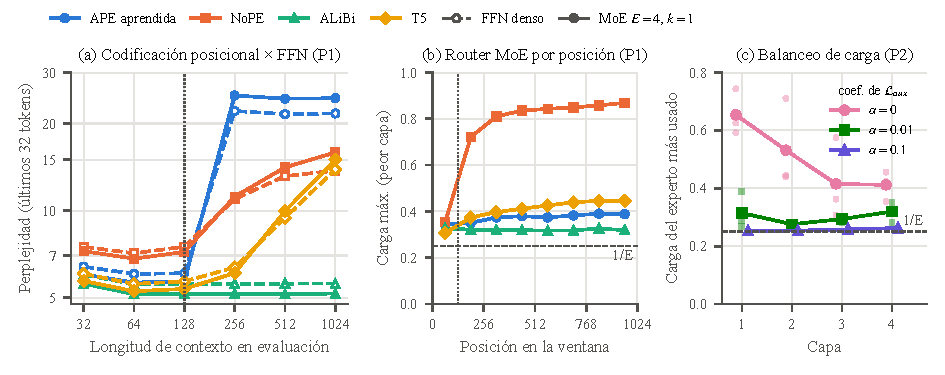
\includegraphics[width=\textwidth]{figuras/fig_principal.pdf}
\caption{(a) Perplejidad según la longitud del contexto, con FFN denso (línea discontinua) y MoE (línea continua); la línea vertical marca el contexto de entrenamiento. (b) Fracción de tokens que recibe el experto más usado (peor capa) en cada tramo de 128 posiciones. (c) Carga del experto más usado en cada capa según el peso de la pérdida de balanceo (los puntos son las semillas). Medias de 3 semillas.}
\label{fig:main}
\end{figure*}

\begin{table}[t]
\centering\small\setlength{\tabcolsep}{3pt}
\begin{tabular}{@{}lccccc@{}}
\toprule
 & \multicolumn{3}{c}{CE val (ctx 128)} & \multicolumn{2}{c}{Perpl. 1024} \\
\cmidrule(lr){2-4}\cmidrule(l){5-6}
Codificación & denso & MoE & $\Delta$ & denso & MoE \\
\midrule
APE aprendida & 1.831 & 1.772 & $-0.059$\pmsd{.010} & 21.66 & 24.45 \\
NoPE & 2.009 & 1.971 & $-0.038$\pmsd{.024} & 13.74 & 15.89 \\
ALiBi & 1.759 & \textbf{1.694} & $-0.065$\pmsd{.007} & 5.60 & \textbf{5.17} \\
T5 & 1.772 & 1.723 & $-0.049$\pmsd{.006} & 13.87 & 15.01 \\
\bottomrule
\end{tabular}
\caption{Montaje P1 con FFN denso y con MoE (4 expertos, $k{=}1$). Media de 3 semillas; $\Delta$ es la diferencia entre el MoE y el denso con la misma semilla.}
\label{tab:combo}
\end{table}

\paragraph{Resultados.}
Repetimos el montaje P1 con el FFN normal y con el MoE para cuatro codificaciones, usando las mismas semillas y la misma máquina para poder comparar por parejas (Tabla~\ref{tab:combo} y Figura~\ref{fig:main}a).
El MoE mejora la CE con las cuatro, entre 0.038 y 0.065 nats, y gana en las 12 parejas.
Sin embargo, con secuencias largas sigue mandando la codificación.
Con ALiBi la mejora se mantiene hasta 1024 tokens (de 5.60 a 5.17). En cambio, con la APE aprendida y con NoPE el MoE es peor que el denso en las tres semillas, y con T5 depende de la semilla.

Lo más interesante apareció al mirar el router (Figura~\ref{fig:main}b).
Con NoPE, el router de la segunda capa (la tercera en una semilla) reparte bien los tokens en las posiciones de entrenamiento, pero manda el 86\% de los tokens de las posiciones 896--1023 a un mismo experto. Con ALiBi, en cambio, ese experto se queda en el 29\%.
Además, la puntuación que el router da a ese experto aumenta con la posición (correlación de 0.52, frente a 0.02 con ALiBi).
Nuestra interpretación es que NoPE calcula internamente una especie de posición absoluta a partir de la máscara causal \citep{kazemnejad2023impact}, y en posiciones que nunca ha visto esa información toma valores nuevos.
Como el router elige un solo experto, basta con que la probabilidad de ese experto suba un poco (de 0.24 a 0.40) para que se lleve casi todos los tokens.

Por último, nuestras ejecuciones del modelo denso dan las mismas medias que las del resto del equipo (diferencias de 0.011 nats como máximo), aunque no los mismos valores semilla a semilla. Por eso solo comparamos ejecuciones hechas en la misma máquina.

\section{Conclusiones y limitaciones}
Las dos ampliaciones resuelven problemas distintos del modelo del libro y se pueden combinar sin cambiar el código de ninguna.
La codificación posicional decide si el modelo funciona con secuencias más largas (ALiBi es la que mejor lo hace), y el MoE mejora el modelo sin aumentar el cálculo por token.
Al juntarlas, el MoE mejora con todas las codificaciones, pero solo mantiene la mejora en secuencias largas con ALiBi.
Como limitaciones, los modelos son muy pequeños, se entrenaron en CPU con un solo corpus a nivel de carácter y no se entrenaron hasta converger.
Con 3 semillas, las diferencias menores de unos 0.01 nats no son concluyentes, y tres de las tareas sintéticas no llegaron a aprenderse.
Además, los tiempos son de CPU, y en GPU un reparto desequilibrado entre expertos sería más costoso.
Como trabajo futuro nos gustaría probar un límite de tokens por experto, los expertos compartidos \citep{dai2024deepseekmoe} y un router que no dependa de la posición.
El código, los tests y los resultados están en la rama feat/moe del repositorio del grupo, y todas las cifras de esta memoria salen de las carpetas results/ y runs/.

\bibliography{referencias}

\end{document}
